\documentclass{beamer}
\setbeamertemplate{navigation symbols}{}
\setbeamertemplate{footline}{}
\usepackage[utf8]{inputenc}
\usepackage{utopia} %font utopia imported
\usetheme{Berlin}
\definecolor{UBCblue}{rgb}{0.04706, 0.13725, 0.26667} % UBC Blue (primary)
\usepackage{wrapfig}

\usecolortheme[named=UBCblue]{structure}%------------------------------------------------------------
\title[MAP 3305] %optional
{Machine Learns To Detect Green and Red Lights Using AlexNet}



\author[Cattan, Dov] % (optional)
{Dov Cattan}

\institute[FAU] % (optional)
{
  
  Student, Computer Engineering\\
  Florida Atlantic University
  
}

\date[ 2022] 
{
 Engineering Math, Spring 2022
\newline \newline 
}




\begin{document}
\frame{\titlepage}

\section{}


\begin{frame}
\frametitle{The importance of Machine Learning as opposed to Machine Memory}








As opposed to memorizing the correct answers on a test, it is more important to learn why the answers are correct. The same applies to AI here, as we use a Convolution Neural Network (CNN) called an AlexNet here to train and test the machine (AI) for accuracy.


  \begin{center}
     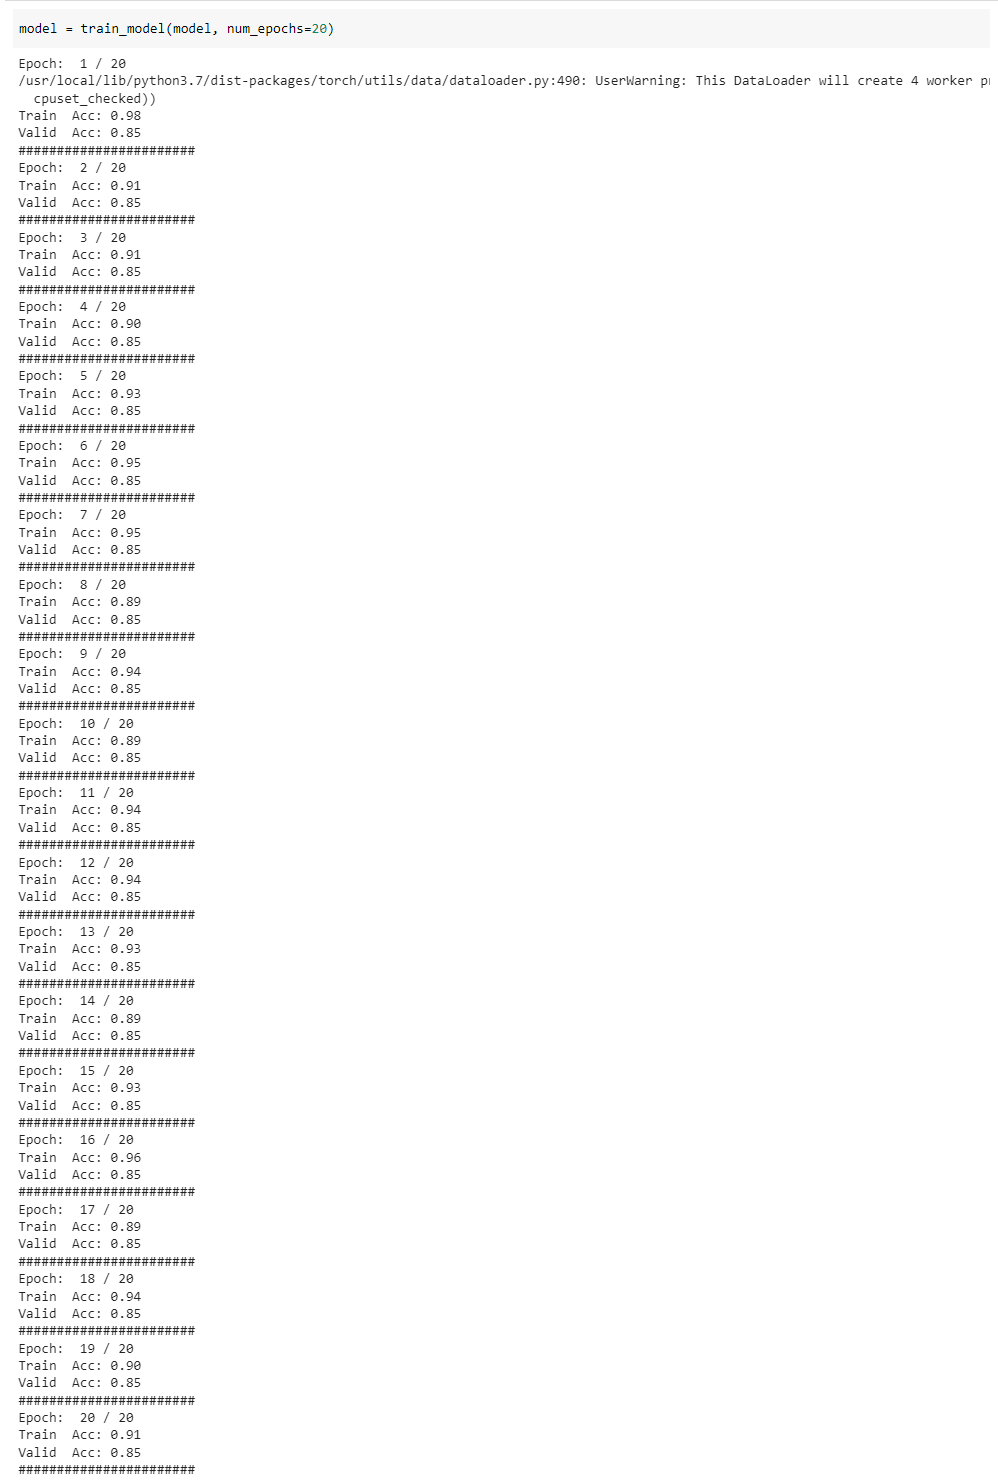
\includegraphics[height = 15cm,width=7.5cm]{training.PNG} 
  \end{center}

\end{frame}



\section{}
%---------------------------------------------------------
%Highlighting text
\begin{frame}

    
  \frametitle{How the Alexnet works}
The Alexnet is a convolution neural network (CNN) architecture, that has convolution, pooling, and ReLU layers that can detect certain pixels from an image that the programmer wants the machine to learn.\newline


   
   \newline
   


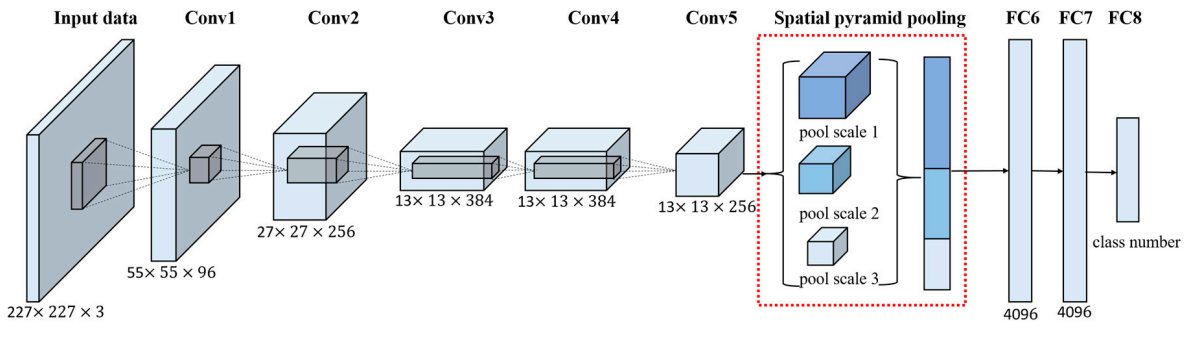
\includegraphics[height = 4.35cm, width= 12cm]{alexnet2.PNG}




\end{frame}
%---------------------------------------------------------


%---------------------------------------------------------
%Two columns
\begin{frame}
\frametitle{How is the Alexnet applied to differentiating traffic light colors}
\begin{minipage}{0.3\textwidth}
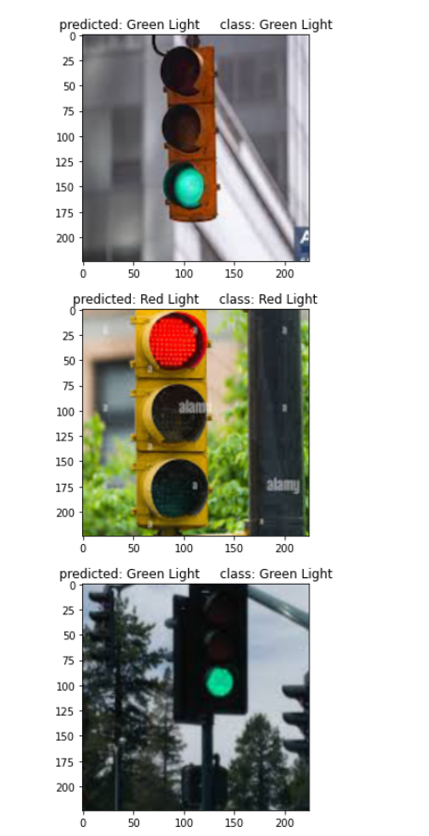
\includegraphics[height =6.25cm,width=3.5cm]{pictures result1.PNG}

\end{minipage}
\begin{minipage}{0.3\textwidth}
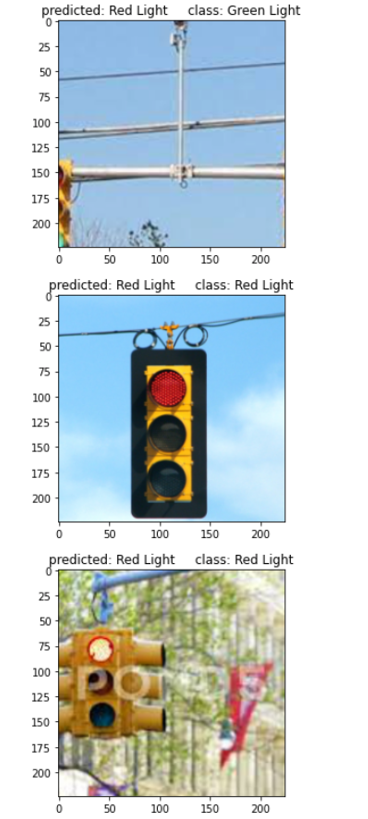
\includegraphics[height =6.25cm,width=3.5cm]{pictures result2.PNG}

\end{minipage}
\begin{minipage}{0.2\textwidth}
From images given to the Alexnet from a dataset, the AI learns to differentiate images of red and green lights, as opposed to memorizing.
\end{minipage}



\newline








\end{frame}
%---------------------------------------------------------
\begin{frame}
\frametitle{References}
Han, Xiaobing, Yanfei Zhong, Liqin Cao, and Liangpei Zhang. 2017. "Pre-Trained AlexNet Architecture with Pyramid Pooling and Supervision for High Spatial Resolution Remote Sensing Image Scene Classification" Remote Sensing 9, no. 8: 848. https://doi.org/10.3390/rs9080848
\end{frame}
\end{document}
